%\begin{appendices}

\appendix
\setcounter{section}{0}% Reset numbering for sections
\renewcommand{\thesection}{\Alph{section}}% Adjust section printing (from here onward)
\renewcommand{\thesubsection}{\Alph{section}.\arabic{subsection}}% Subsections of appendix: H.1, H.2 (not 0.8.1)
\renewcommand{\thesubsubsection}{\Alph{section}.\arabic{subsection}.\arabic{subsubsection}}

% Bloque unificado de anexos en orientacion horizontal (Arbol de Problemas,
% Arbol de Objetivos y Matriz de Consistencia). Se usa un solo entorno
% \begin{landscape} para evitar paginas en blanco entre cada anexo y se
% aplica el pagestyle 'horizontal' que oculta el encabezado largo (que no
% entra correctamente al rotar la pagina) dejando unicamente el numero de
% pagina al pie.

\begin{landscape} 
% ──────────────────────────────────────────────────────────────
\section{Árbol de Problemas}
% ──────────────────────────────────────────────────────────────

\label{anexo1}

\begin{figure}[H]
	\centering
	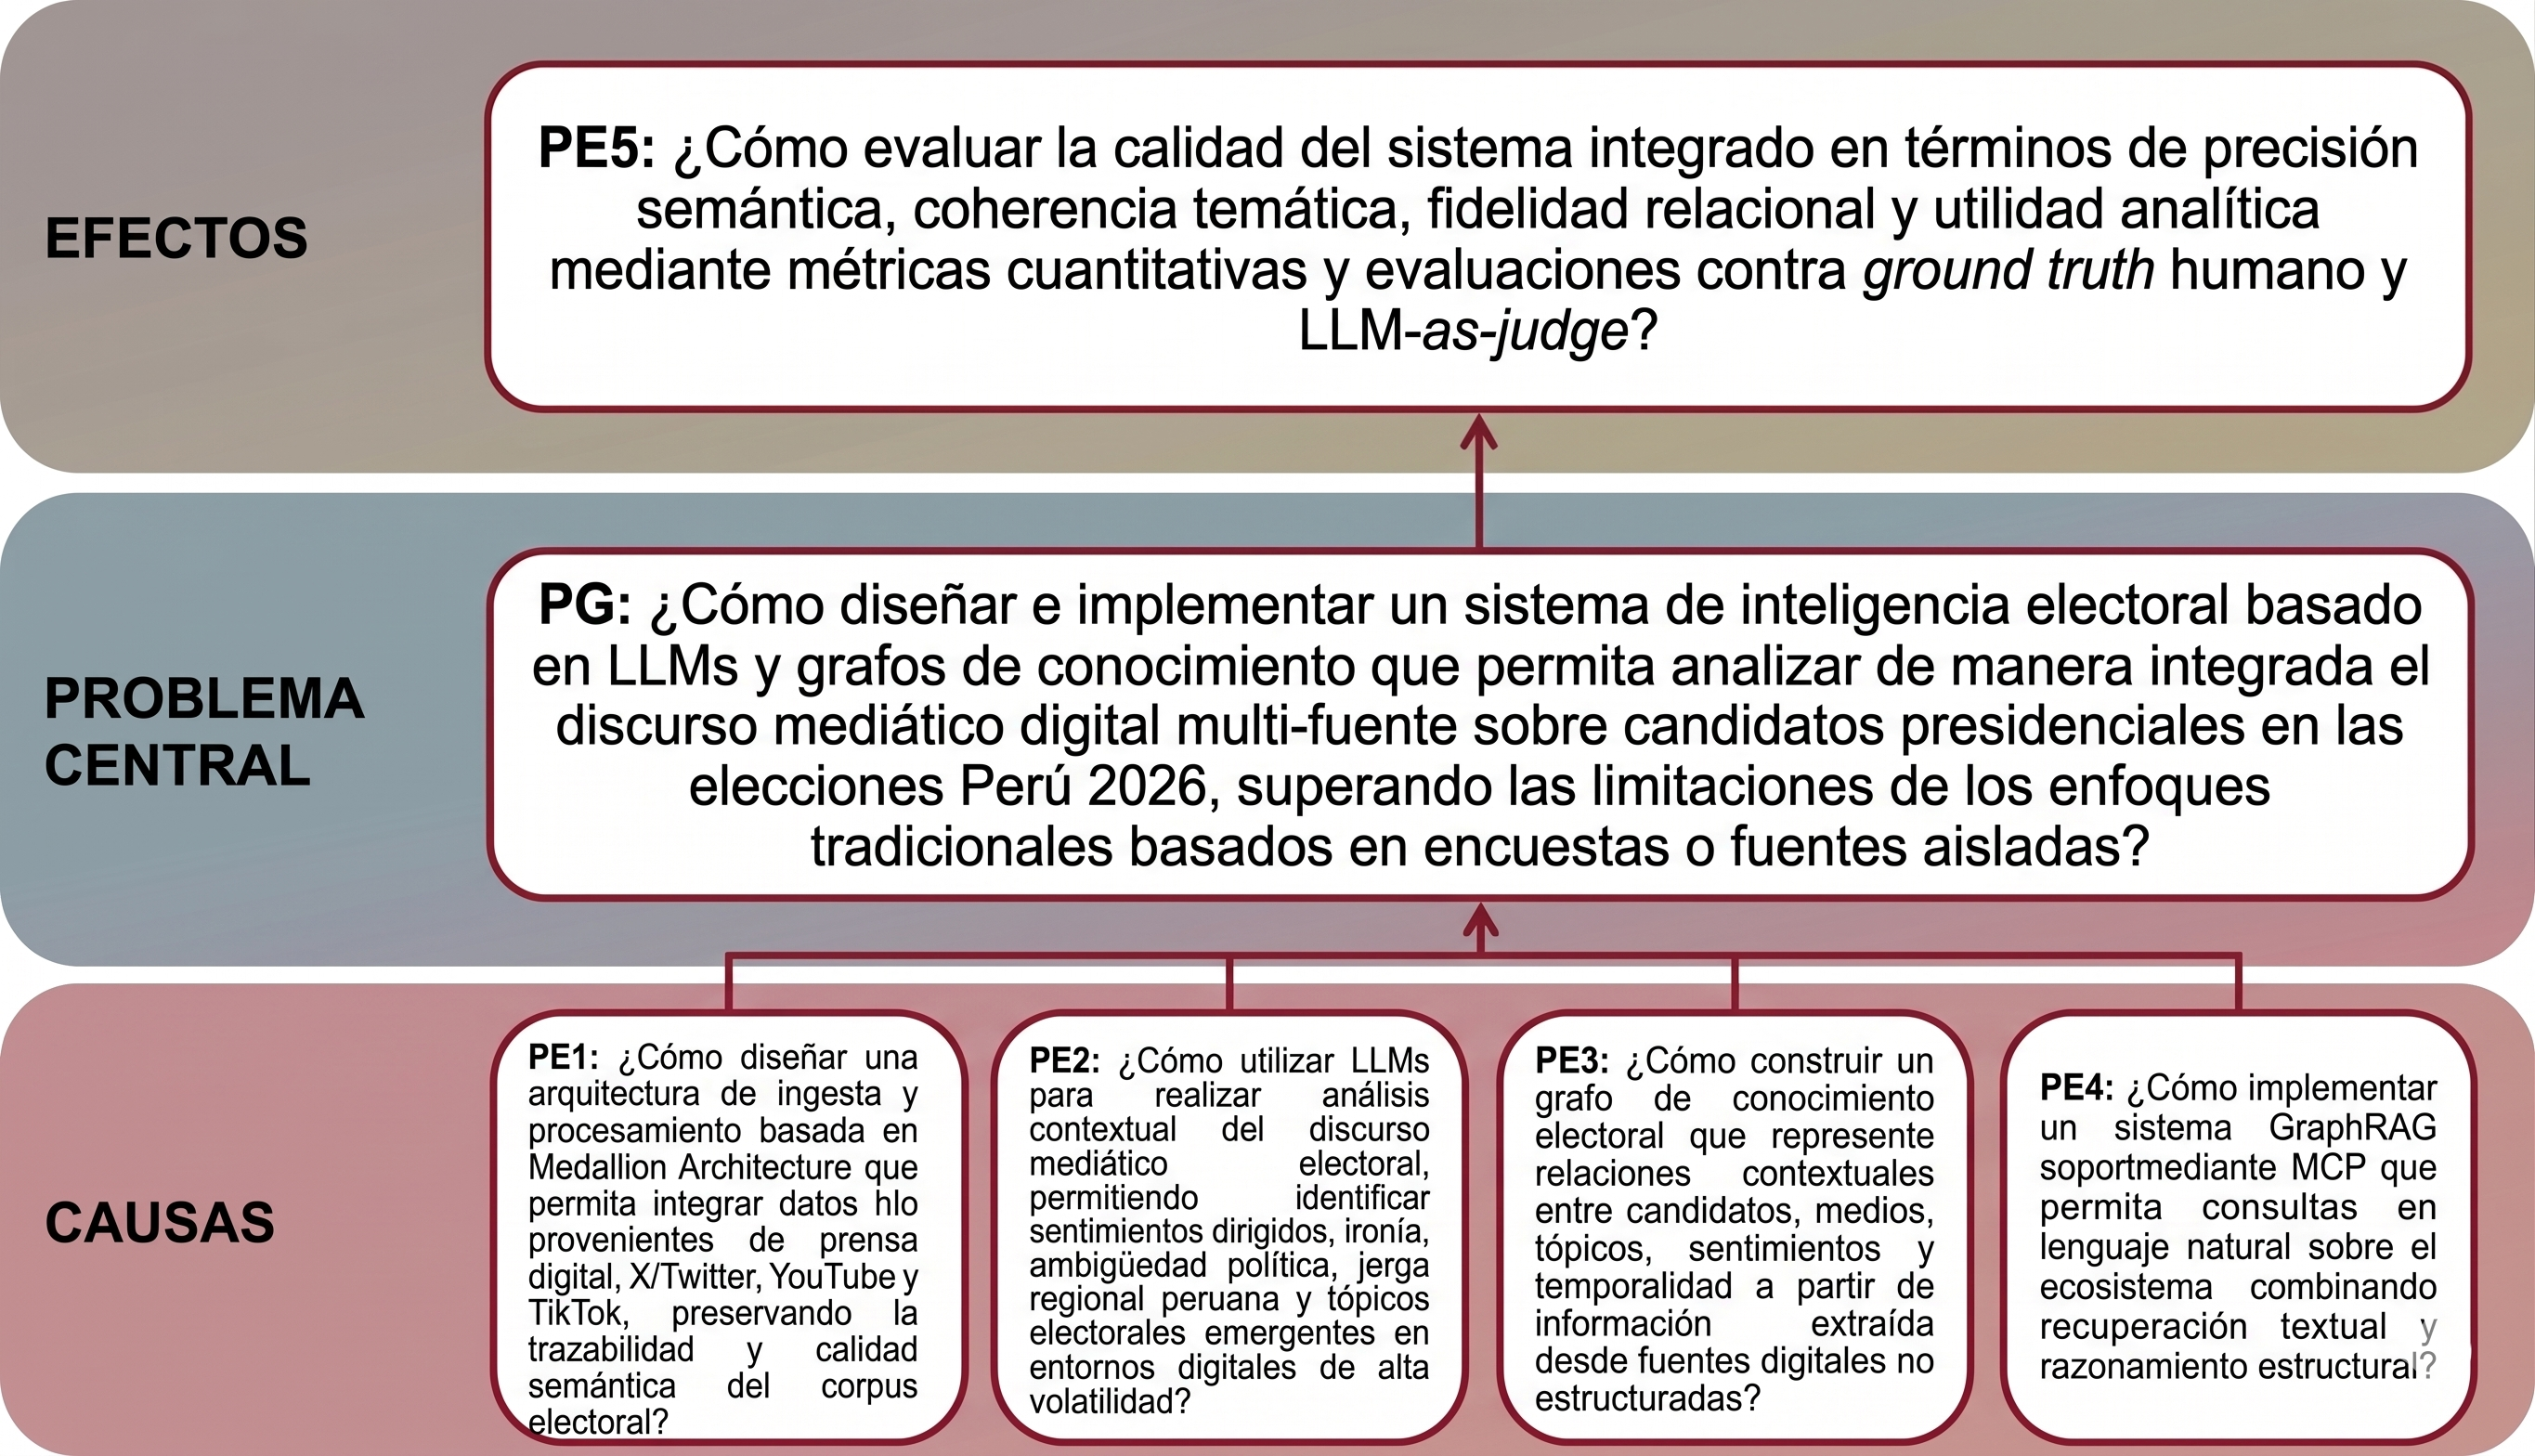
\includegraphics[width=1.15\textwidth]{anexos/arbol_problemas.png}
	\caption[Árbol de problemas de la investigación]{Árbol de problemas identificados en la investigación sobre análisis de la percepción actual proyectada por los medios de comunicación en contextos electorales mediante inteligencia electoral.\\
	Fuente: Elaboración propia.}
	\label{fig:arbol_problemas}
\end{figure}

\newpage

% ──────────────────────────────────────────────────────────────
\section{Árbol de Objetivos}
% ──────────────────────────────────────────────────────────────

\label{anexo2}

\begin{figure}[H]
	\centering
	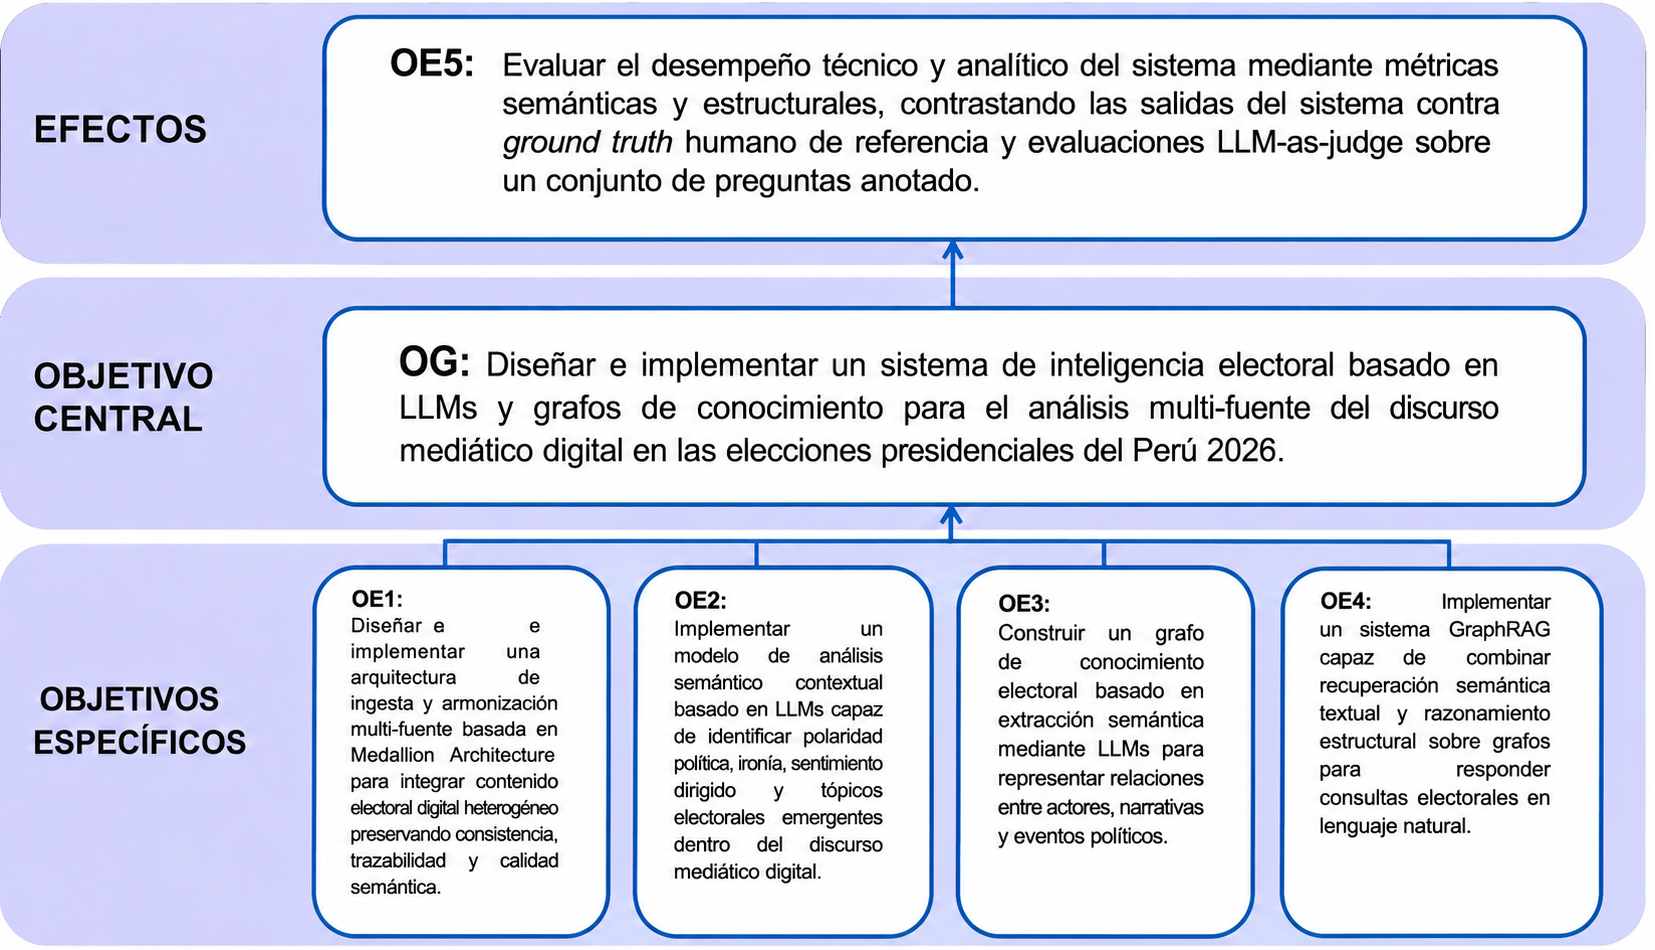
\includegraphics[width=1.15\textwidth]{anexos/arbol_objetivos.png}
	\caption[Árbol de objetivos de la investigación]{Árbol de objetivos que estructuran la investigación sobre análisis de percepciones con LLMs y detección dinámica de temas en ecosistemas digitales.\\
	Fuente: Elaboración propia.}
	\label{fig:arbol_objetivos}
\end{figure}

\newpage

% ──────────────────────────────────────────────────────────────
\section{Matriz de Consistencia}
% ──────────────────────────────────────────────────────────────

\label{anexo3}

\begin{figure}[H]
	\centering
	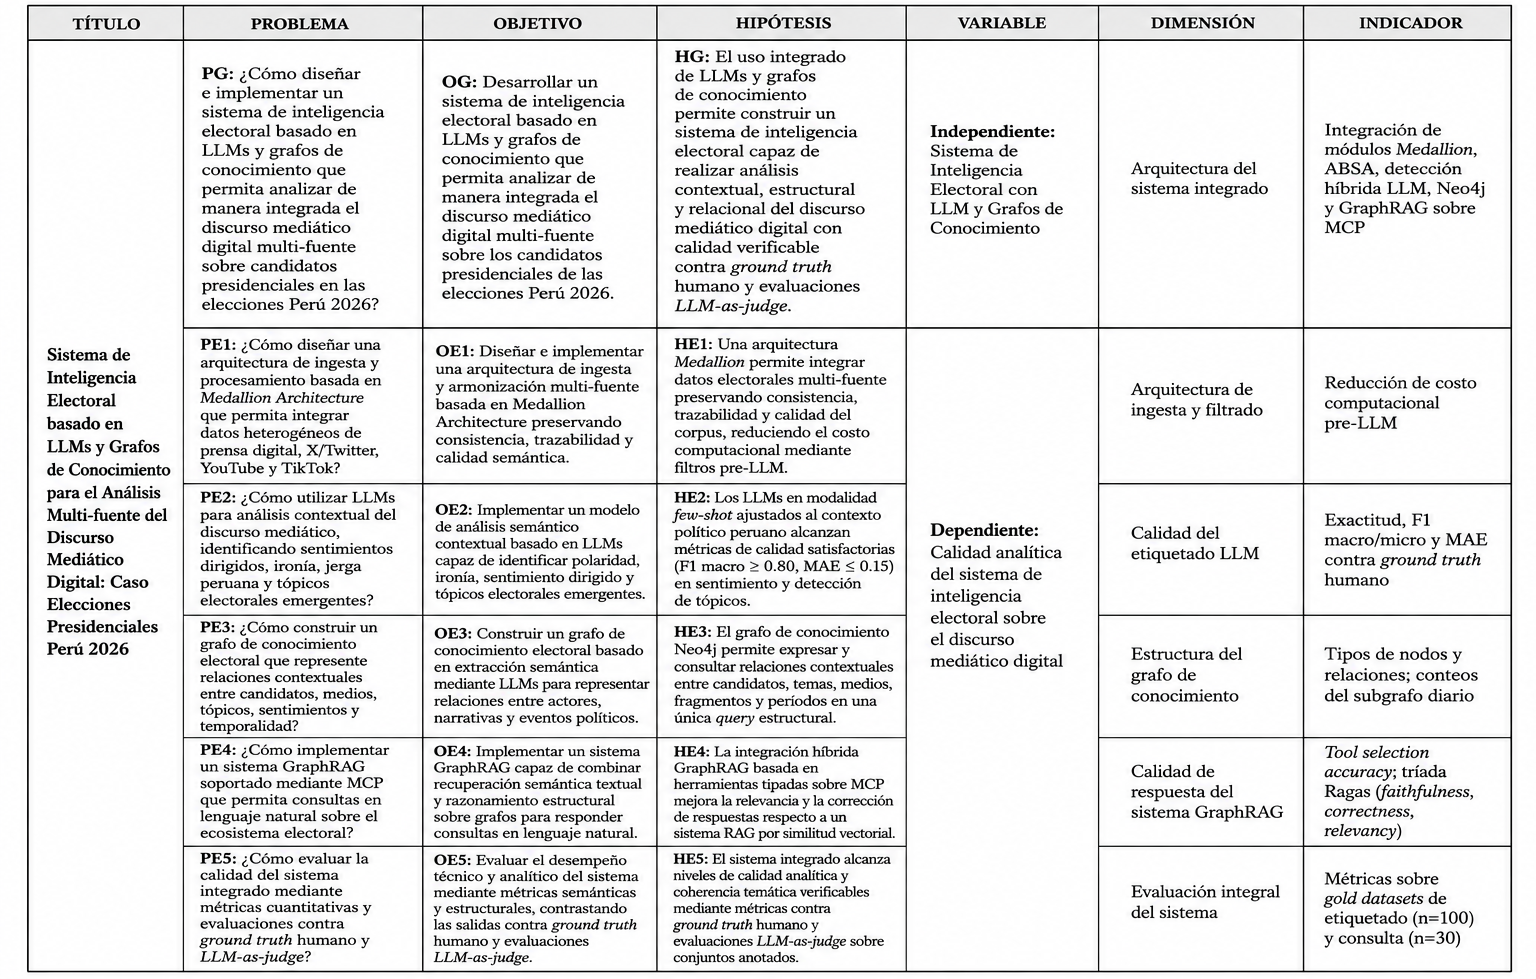
\includegraphics[width=1.15\textwidth]{anexos/matriz_consistencia.png}
	\caption[Matriz de consistencia]{Matriz que muestra la consistencia entre los objetivos, hipótesis y metodología de la investigación.\\
	Fuente: Elaboración propia.}
	\label{fig:matriz_consistencia}
\end{figure}
\end{landscape}
\clearpage

% ──────────────────────────────────────────────────────────────
\section{Configuración de Parámetros del Módulo ABSA con LLM}
% ──────────────────────────────────────────────────────────────

\label{anexo4}

\begin{table}[h]
	\centering	
	\small
	\begin{tabular}{p{4cm} p{5cm} p{4cm}}
		\specialrule{.1em}{.05em}{.05em}
		\textbf{Parámetro} & \textbf{Valor/Configuración} & \textbf{Justificación} \\
		\specialrule{.1em}{.05em}{.05em}
		
		Modelo LLM & DeepSeek-Chat (principal) / Gemini Flash (fallback) & DeepSeek ofrece caché de prefijo (ahorro \textasciitilde 75\% en tokens de entrada) y soporte nativo de \texttt{response\_format: JSON}; Gemini Flash queda como fallback configurable vía \texttt{LLM\_PROVIDER} \\
		\hline
		
		Rol del Prompt & Analista político experto & Orienta el modelo hacia el dominio electoral latinoamericano \\
		\hline
		
		Ejemplos \textit{Few-Shot} & 4 ejemplos & De acuerdo con \cite{pr_gujral2024llm_elections}, mínimo 3 ejemplos mejora precisión en contextos no anglosajones \\
		\hline
		
		Escala de Sentimiento & Continua $[-1, 1]$ & Captura intensidad del sentimiento más allá de polaridad binaria \\
		\hline
		
		Umbral Clasificación & Positivo: $S > 0.2$, Negativo: $S < -0.2$, Neutro: $[-0.2, 0.2]$ & Reduce ruido de sentimientos débiles \\
		\hline
		
		Estrategia \textit{Early Stopping} & 3 iteraciones sin mejora F1 & Evita sobreajuste y desperdicio de tokens API \\
		\hline
		
		Formato de Respuesta & JSON con validación esquema & Estructuración consistente de candidatos, sentimientos, temas y relaciones \\
		\hline
		
		Temperatura/Creatividad & Baja (0.2-0.3) & Reproducibilidad y consistencia en clasificación \\
		
		\specialrule{.1em}{.05em}{.05em}
	\end{tabular}
	\caption[Configuración de parámetros del módulo ABSA]{Parámetros finales configurados para el módulo de análisis de sentimientos a nivel de aspecto (ABSA) usando DeepSeek-Chat como proveedor principal y Gemini Flash como fallback.}
	\label{tbl:config_absa}
\end{table}

\clearpage

% ──────────────────────────────────────────────────────────────
\section{Configuración del Módulo Híbrido LLM con Catálogo Incremental}
% ──────────────────────────────────────────────────────────────

\label{anexo5}

\begin{table}[h]
	\centering
	\small
	\begin{tabular}{p{4cm} p{5cm} p{4cm}}
		\specialrule{.1em}{.05em}{.05em}
		\textbf{Parámetro} & \textbf{Valor} & \textbf{Justificación} \\
		\specialrule{.1em}{.05em}{.05em}

		Modelo Embedding & \texttt{paraphrase-multilingual-mpnet-base-v2} & Mejor balance entre calidad semántica y velocidad para español \cite{mc_reimers2019sbert} \\
		\hline

		Dimensión Embedding & 768 & Dimensión estándar del modelo multilingüe seleccionado \\
		\hline

		Almacén Vectorial & PostgreSQL + pgvector & Búsqueda por similitud cosine sobre el catálogo incremental de temas \\
		\hline

		Tamaño del Menú & Hasta 20 candidatos & Tope superior del retrieval multinivel inyectado al \textit{prompt} del LLM \\
		\hline

		Tiers de Retrieval & 5 (trending, semántico, léxico, actor, evento) & Maximiza la cobertura del menú combinando señales heterogéneas \\
		\hline

		Clasificación LLM & \texttt{exact} / \texttt{alias} / \texttt{new} & El LLM decide reusar tema existente, marcarlo como alias o crear uno nuevo \\
		\hline

		Override Semántico & Cosine $\geq 0.85$ post-LLM & Captura duplicados que escapan al menú de retrieval \\
		\hline

		Consolidación Diaria & Threshold cosine $\geq 0.78$ & Fusiona temas semánticamente equivalentes generados en el día \\
		\hline

		\texttt{llm\_dedup\_day} & Máx. 200 pares/día & Deduplicación con LLM Juez sobre pares sospechosos, acotada por costo \\

		\specialrule{.1em}{.05em}{.05em}
	\end{tabular}
	\caption[Configuración del módulo híbrido LLM con catálogo incremental]{Parámetros de configuración del módulo híbrido LLM con catálogo incremental para la detección dinámica de temas electorales sobre el corpus multicanal.}
	\label{tbl:config_temas_hibrido}
\end{table}

\clearpage

% ──────────────────────────────────────────────────────────────
\section{Esquema del Grafo de Conocimiento Electoral en Neo4j}
% ──────────────────────────────────────────────────────────────

\label{anexo6}

\begingroup
\renewcommand\arraystretch{1.3}
\small
\setlength{\LTpost}{0pt}

\begin{longtable}{p{2.6cm} p{4.2cm} p{5.5cm}}
    \caption[Esquema del grafo de conocimiento electoral]{Especificación completa de nodos, propiedades y relaciones implementadas en el grafo de conocimiento electoral en Neo4j 5.20 Community Edition (con plugins GDS y APOC).} \label{tbl:esquema_grafo} \\

    \specialrule{.1em}{.05em}{.05em}
    \centering\textbf{TIPO NODO} & \centering\textbf{PROPIEDADES} & \centering\arraybackslash\textbf{DESCRIPCIÓN} \\
    \specialrule{.1em}{.05em}{.05em}
    \endfirsthead

    \specialrule{.1em}{.05em}{.05em}
    \centering\textbf{TIPO NODO} & \centering\textbf{PROPIEDADES} & \centering\arraybackslash\textbf{DESCRIPCIÓN} \\
    \specialrule{.1em}{.05em}{.05em}
    \endhead

    Documento & id, uid, fuente, tipo, titulo, url, publicado\_en & Publicaciones del corpus multifuente (noticia, twitter, youtube, tiktok) \\ \hline
    Fragmento & id, texto, embedding (768D), fecha & Segmento textual extraído del documento, indexado vectorialmente \\ \hline
    Tema & id, nombre, categoria, embedding (768D) & Temas emergentes detectados por el módulo híbrido LLM con catálogo incremental \\ \hline
    Actor & id (slug), nombre, tipo, embedding (768D) & Actores institucionales o ad-hoc detectados en el corpus \\ \hline
    Candidato & id (slug), nombre, partido, espectro\_politico, embedding (768D) & Candidatos presidenciales del proceso electoral \\ \hline
    Categoria & nombre & Categoría temática del catálogo cerrado de 17 valores \\ \hline
    Encuesta & id, encuestadora, fecha\_publicacion, n\_muestra, margen\_error & Encuestas electorales con metadatos completos \\ \hline
    SentimientoDiario & id, fecha, actor\_id, sentimiento\_avg, n\_menciones & Agregado diario del sentimiento mediático por candidato \\ \hline
    TipoCambio & fecha, moneda, compra, venta, promedio & Tipo de cambio diario (BCRP) \\ \hline
    IndicadorMacro & fecha, indicador, valor, unidad & Indicadores macroeconómicos (IGBVL var \%, EMBI Perú) \\ \hline

    \specialrule{.1em}{.05em}{.05em}
    \textbf{TIPO RELACIÓN} & \multicolumn{2}{p{10cm}}{\centering\textbf{METADATOS Y DESCRIPCIÓN}} \\
    \specialrule{.1em}{.05em}{.05em}

    CONTIENE & (sin propiedades) & Documento contiene Fragmento \\ \hline
    SOBRE\_TEMA & sentimiento, confianza & Fragmento trata sobre un Tema \\ \hline
    MENCIONA & sentimiento, rol & Fragmento menciona a un Candidato con un sentimiento dado \\ \hline
    MENCIONA\_ACTOR & rol & Fragmento menciona a un Actor (institucional o ad-hoc) \\ \hline
    DE\_CATEGORIA & (sin propiedades) & Tema pertenece a una Categoria del catálogo cerrado \\ \hline
    MIDE & intencion\_voto, posicion\_ranking & Encuesta mide la intención de voto de un Candidato \\ \hline
    TIENE\_SENTIMIENTO\_EN & (sin propiedades) & Candidato tiene un agregado SentimientoDiario en una fecha \\
    \specialrule{.1em}{.05em}{.05em}
\end{longtable}
\endgroup

\clearpage

% ──────────────────────────────────────────────────────────────
\section{Diccionario de Palabras Clave Electorales}
% ──────────────────────────────────────────────────────────────

\label{anexo7}

\begingroup
\renewcommand\arraystretch{1.3}
\small
\setlength{\LTpost}{0pt}

\begin{longtable}{p{3cm} p{7cm} p{3cm}}
	\caption[Diccionario de palabras clave electorales]{Vocabulario controlado utilizado para filtrar publicaciones relevantes en el corpus multi-fuente durante el período de análisis electoral.} \label{tbl:diccionario_palabras_clave} \\

	\specialrule{.1em}{.05em}{.05em}
	\centering\textbf{CATEGORÍA} & \centering\textbf{TÉRMINOS} & \centering\arraybackslash\textbf{CANTIDAD} \\
	\specialrule{.1em}{.05em}{.05em}
	\endfirsthead

	\specialrule{.1em}{.05em}{.05em}
	\centering\textbf{CATEGORÍA} & \centering\textbf{TÉRMINOS} & \centering\arraybackslash\textbf{CANTIDAD} \\
	\specialrule{.1em}{.05em}{.05em}
	\endhead

	Procesos Electorales & elección, voto, votación, candidato, campaña, debate, mitin, encuesta, sondeo & 9 \\ \hline
	Términos Políticos & gobierno, política, legislatura, congreso, república, democracia, parlamento & 7 \\ \hline
	Instituciones & ONPE, JNE, RENIEC, INE, INEI, MINDEF & 6 \\ \hline
	Temas de Campaña & economía, seguridad, educación, salud, corrupción, gobernabilidad, infraestructura & 7 \\ \hline
	Hashtags Electorales & \#EleccionesPerú2026, \#Voto2026, \#DebatePresidencial, \#CuéntaTuVoto & 4+ \\ \hline
	Candidatos & Nombres completos, apodos, siglas de partidos & Dinámico según proceso \\
	\specialrule{.1em}{.05em}{.05em}
\end{longtable}
\endgroup

\clearpage

% ──────────────────────────────────────────────────────────────
\section{Métodos Estadísticos para Validación de Modelos}
% ──────────────────────────────────────────────────────────────

\label{anexo8}

\subsection{Métricas de Desempeño para ABSA}

Para la evaluación del módulo de análisis de sentimientos a nivel de aspecto, se emplearon las siguientes métricas estadísticas en escala $[0, 1]$:

\begin{equation}
\text{Exactitud} = \frac{\text{TP} + \text{TN}}{\text{TP} + \text{TN} + \text{FP} + \text{FN}}
\end{equation}

\begin{equation}
\text{Precisión} = \frac{\text{TP}}{\text{TP} + \text{FP}}
\end{equation}

\begin{equation}
\text{Cobertura (Recall)} = \frac{\text{TP}}{\text{TP} + \text{FN}}
\end{equation}

\begin{equation}
\text{F1-Score Macro} = \frac{1}{n}\sum_{i=1}^{n}\frac{2 \cdot \text{Precisión}_i \cdot \text{Cobertura}_i}{\text{Precisión}_i + \text{Cobertura}_i}
\end{equation}

Donde TP (Verdaderos Positivos), TN (Verdaderos Negativos), FP (Falsos Positivos), FN (Falsos Negativos) representan los conteos de clasificación por clase.

\clearpage

% ──────────────────────────────────────────────────────────────
\section{Timeline Experimental de CRISP-DM}
% ──────────────────────────────────────────────────────────────

\label{anexo9}

\begin{table}[h]
	\centering
	\small
	\begin{tabular}{p{2.5cm} p{3.5cm} p{2.5cm} p{4cm}}
		\specialrule{.1em}{.05em}{.05em}
		\centering\textbf{FASE} & \centering\textbf{ACTIVIDADES CLAVE} & \centering\textbf{DURACIÓN} & \centering\arraybackslash\textbf{ENTREGABLES} \\
		\specialrule{.1em}{.05em}{.05em}
		
		1. Comprensión del Negocio & Definición de problema, objetivos e hipótesis; Revisión de literatura & 2 semanas & Documento de especificaciones \\
		\hline
		
		2. Comprensión de Datos & Construcción de corpus (noticias digitales, X/Twitter, YouTube, TikTok); Análisis exploratorio & 3 semanas & Datasets en capas Bronze y Silver \\
		\hline
		
		3. Preparación de Datos & Limpieza, normalización, tokenización; Segmentación por período & 2 semanas & Corpus preprocesado validado \\
		\hline
		
		4. Modelamiento & Config. ABSA, módulo híbrido LLM, Neo4j, GraphRAG; Calibración de parámetros & 4 semanas & Modelos entrenados y validados \\
		\hline
		
		5. Evaluación & Métricas de desempeño, análisis comparativo, validación cualitativa & 2 semanas & Reporte de resultados \\
		\hline
		
		6. Despliegue & Prototipo funcional con datos en tiempo real; Documentación técnica & 1 semana & Sistema operacional \\
		
		\specialrule{.1em}{.05em}{.05em}
	\end{tabular}
	\caption[Timeline experimental de las fases CRISP-DM]{Cronograma de implementación de las seis fases de la metodología CRISP-DM aplicada en la investigación.}
	\label{tbl:timeline_crisp_dm}
\end{table}


